\section{Runtime and Memory Architecture}
\label{sec:runtime}

\begin{figure}[t]
  \centering
  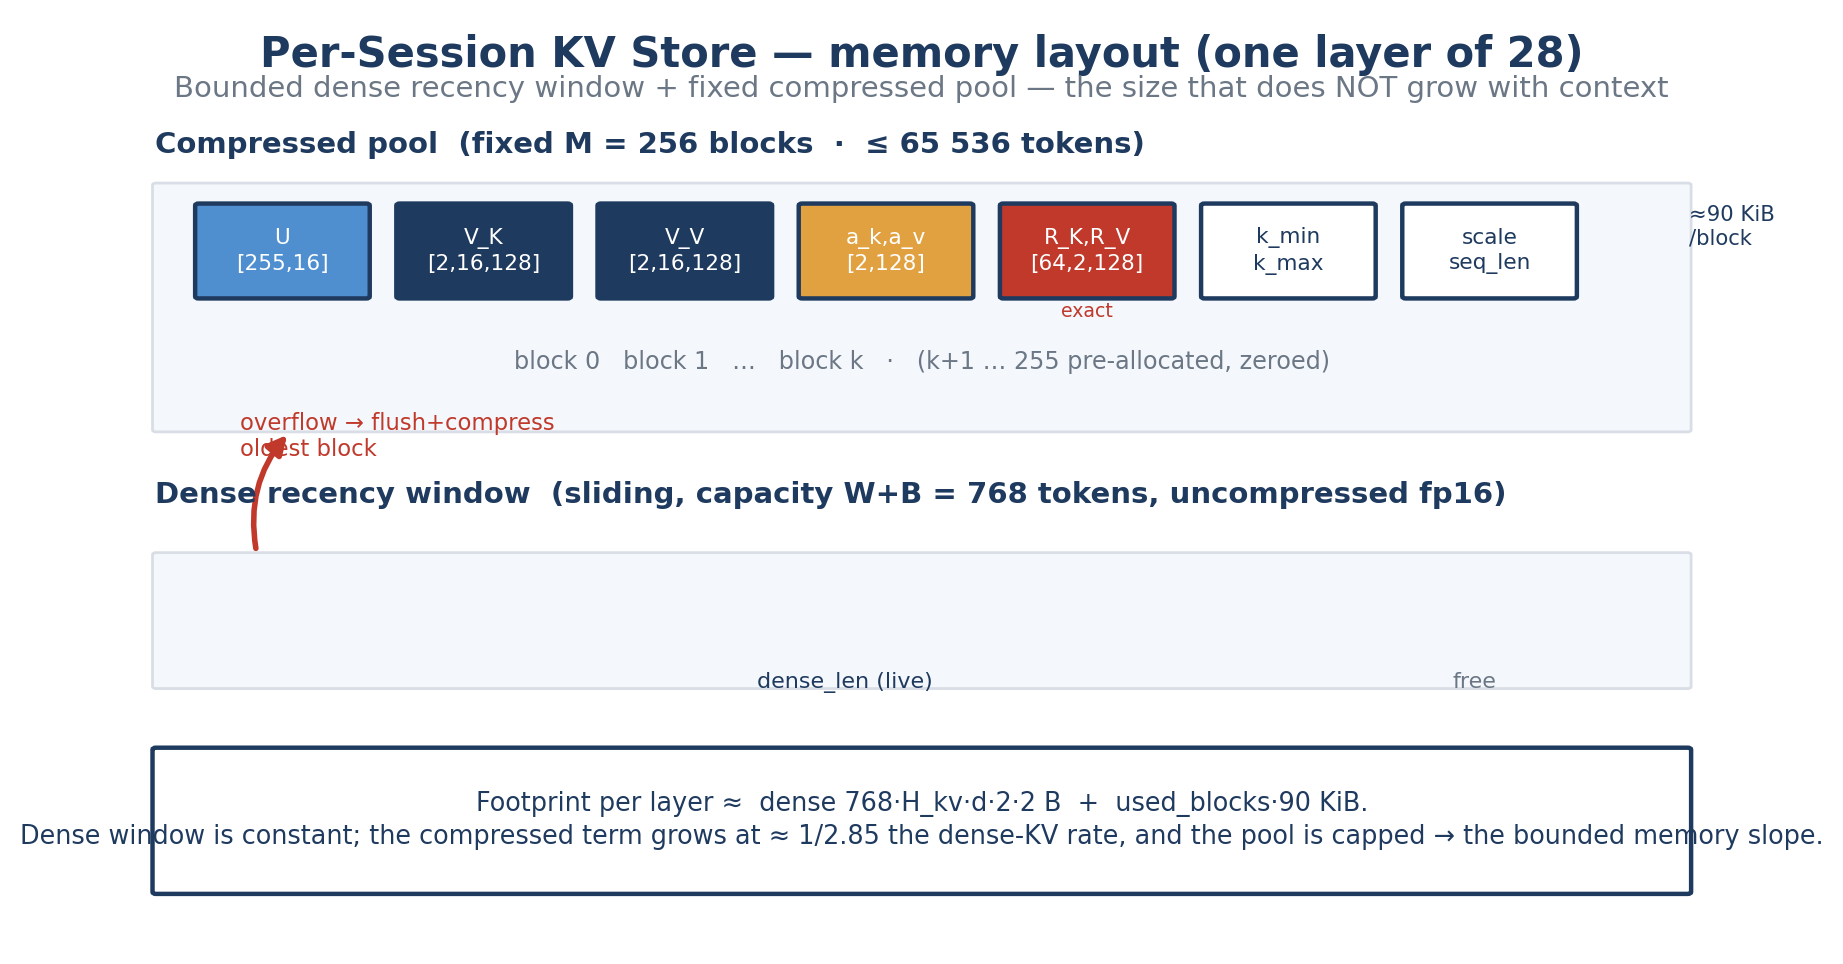
\includegraphics[width=\linewidth]{figures/f3_memory_layout.png}
  \caption{Per-session KV store (one of $28$ layers). A fixed compressed pool of $M{=}256$
  blocks (pre-allocated, zero-filled) plus a sliding dense recency window of capacity
  $\dwin{+}\bs{=}768$ tokens. The pool's footprint is independent of context length; the
  window is bounded. Overflowing the window compresses its oldest block into the pool.}
  \label{fig:layout}
\end{figure}

\subsection{Per-session state}
For each session and layer the manager holds (Fig.~\ref{fig:layout}):
a dense window $K^{\text{win}},V^{\text{win}}\in\R^{\Hkv\times 768\times\dhead}$ (fp16) with a
fill counter; and a compressed pool of $M{=}256$ pre-allocated slots, each holding the low-rank
factors $\{U,V_K,V_V,\anchork,\anchorv,s\}$, the $\maxres{=}64$ exact residual KV pairs
$\{R_K,R_V\}$, and the router's key min/max $\{k^{\min},k^{\max}\}$ (\S\ref{sec:compression}).
Pre-allocation matters: the pool occupies its full footprint from the start, so memory does not
fragment or spike as blocks are added, and the store's size is a \emph{constant} of the
configuration---$M\bs{=}65{,}536$ compressed tokens plus a $768$-token window, $\approx\!0.68$\,GB
across all $28$ layers---not a function of $N$. This is exactly why the runtime can address a
$64$k context: $65{,}536+768 \ge 65{,}615$, the largest prompt we test.

\subsection{Chunked, exact prefill with streaming compression}
Prefill is processed in chunks of $512$ tokens (Alg.~\ref{alg:prefill}). Each chunk is a
forward pass through the patched model using a \emph{native} MLX cache, so a chunk attends
over all prior tokens and the hidden states are numerically exact---\diffkv{} introduces no
approximation during prefill. After the exact attention, the chunk's rotated keys and values
are captured token-by-token into the dense window; whenever the window would overflow its
$768$-token capacity, the oldest $256$-token block is compressed out
(Alg.~\ref{alg:compress}) and the remaining tokens slide forward. Compression is thus
\emph{streamed} during prefill rather than deferred, bounding the window throughout.

\begin{algorithm}[t]
\caption{Prefill (per chunk) and the prefill$\to$decode boundary}
\label{alg:prefill}
\begin{algorithmic}[1]
\For{each $512$-token chunk}
  \State exact SDPA over native cache (attends all prior tokens)
  \For{each token $t$ in chunk, each layer $\ell$}
    \State append $(K_t,V_t)$ to dense window of $\ell$
    \If{window full} \textsc{CompressBlock} oldest $256$; slide window \EndIf
  \EndFor
\EndFor
\State \textbf{boundary:} \texttt{mx.eval}; \texttt{mx.clear\_cache}; \texttt{gc}
\State resolve decode policy (adaptive: compressed iff $N\!\ge\!16$k)
\If{compressed} \textbf{drop native prefill cache} \Comment{decode reads the DiffKV store only} \EndIf
\end{algorithmic}
\end{algorithm}

\subsection{The prefill$\to$decode boundary and the adaptive decode policy}
\label{sec:autopolicy}
At the first decode step the runtime flushes pending lazy work and calls
\texttt{mx.clear\_cache()} and \texttt{gc.collect()} to return the peak GQA-expanded prefill
activations to the OS. It then resolves, \emph{once}, which decode path to use, and stores the
decision for the whole generation. The default policy is \emph{adaptive}: below a context
threshold ($16$k tokens) it keeps the native full-KV cache and decodes exactly---faster, and
memory-safe because the cache is still small---and at or above the threshold it
\emph{drops the native prefill cache entirely} and serves decode from the compressed pool plus
the recency window. The policy reflects the trade-off this paper quantifies: the compressed
kernel's value is a bounded decode-time footprint at long context, exactly the regime where
retaining a full cache through a long generation risks exhausting memory; at short context the
fused full-KV path is both faster and safe, so decode never regresses for ordinary requests. The
threshold and a force-on/force-off override are exposed as environment variables, and our
evaluation reports both forced modes as well as this adaptive default. Dropping the cache is what
makes decode-time memory reflect the compressed store rather than a retained full-context cache;
it is also why, as \S\ref{sec:eval} shows, the global allocator peak (set during prefill) and the
steady-state decode footprint differ.

\subsection{Decode-step bookkeeping}
Each decode step ingests the new token's rotated key and value into the dense window
\emph{before} attention is computed (so the query can attend to itself), then compresses any
block that pushes the window past $\dwin{+}\bs$. The fused attention
(\S\ref{sec:decode}) then runs over the pool and the window. Figure~\ref{fig:lifecycle}
summarizes the full lifecycle.

\begin{figure}[t]
  \centering
  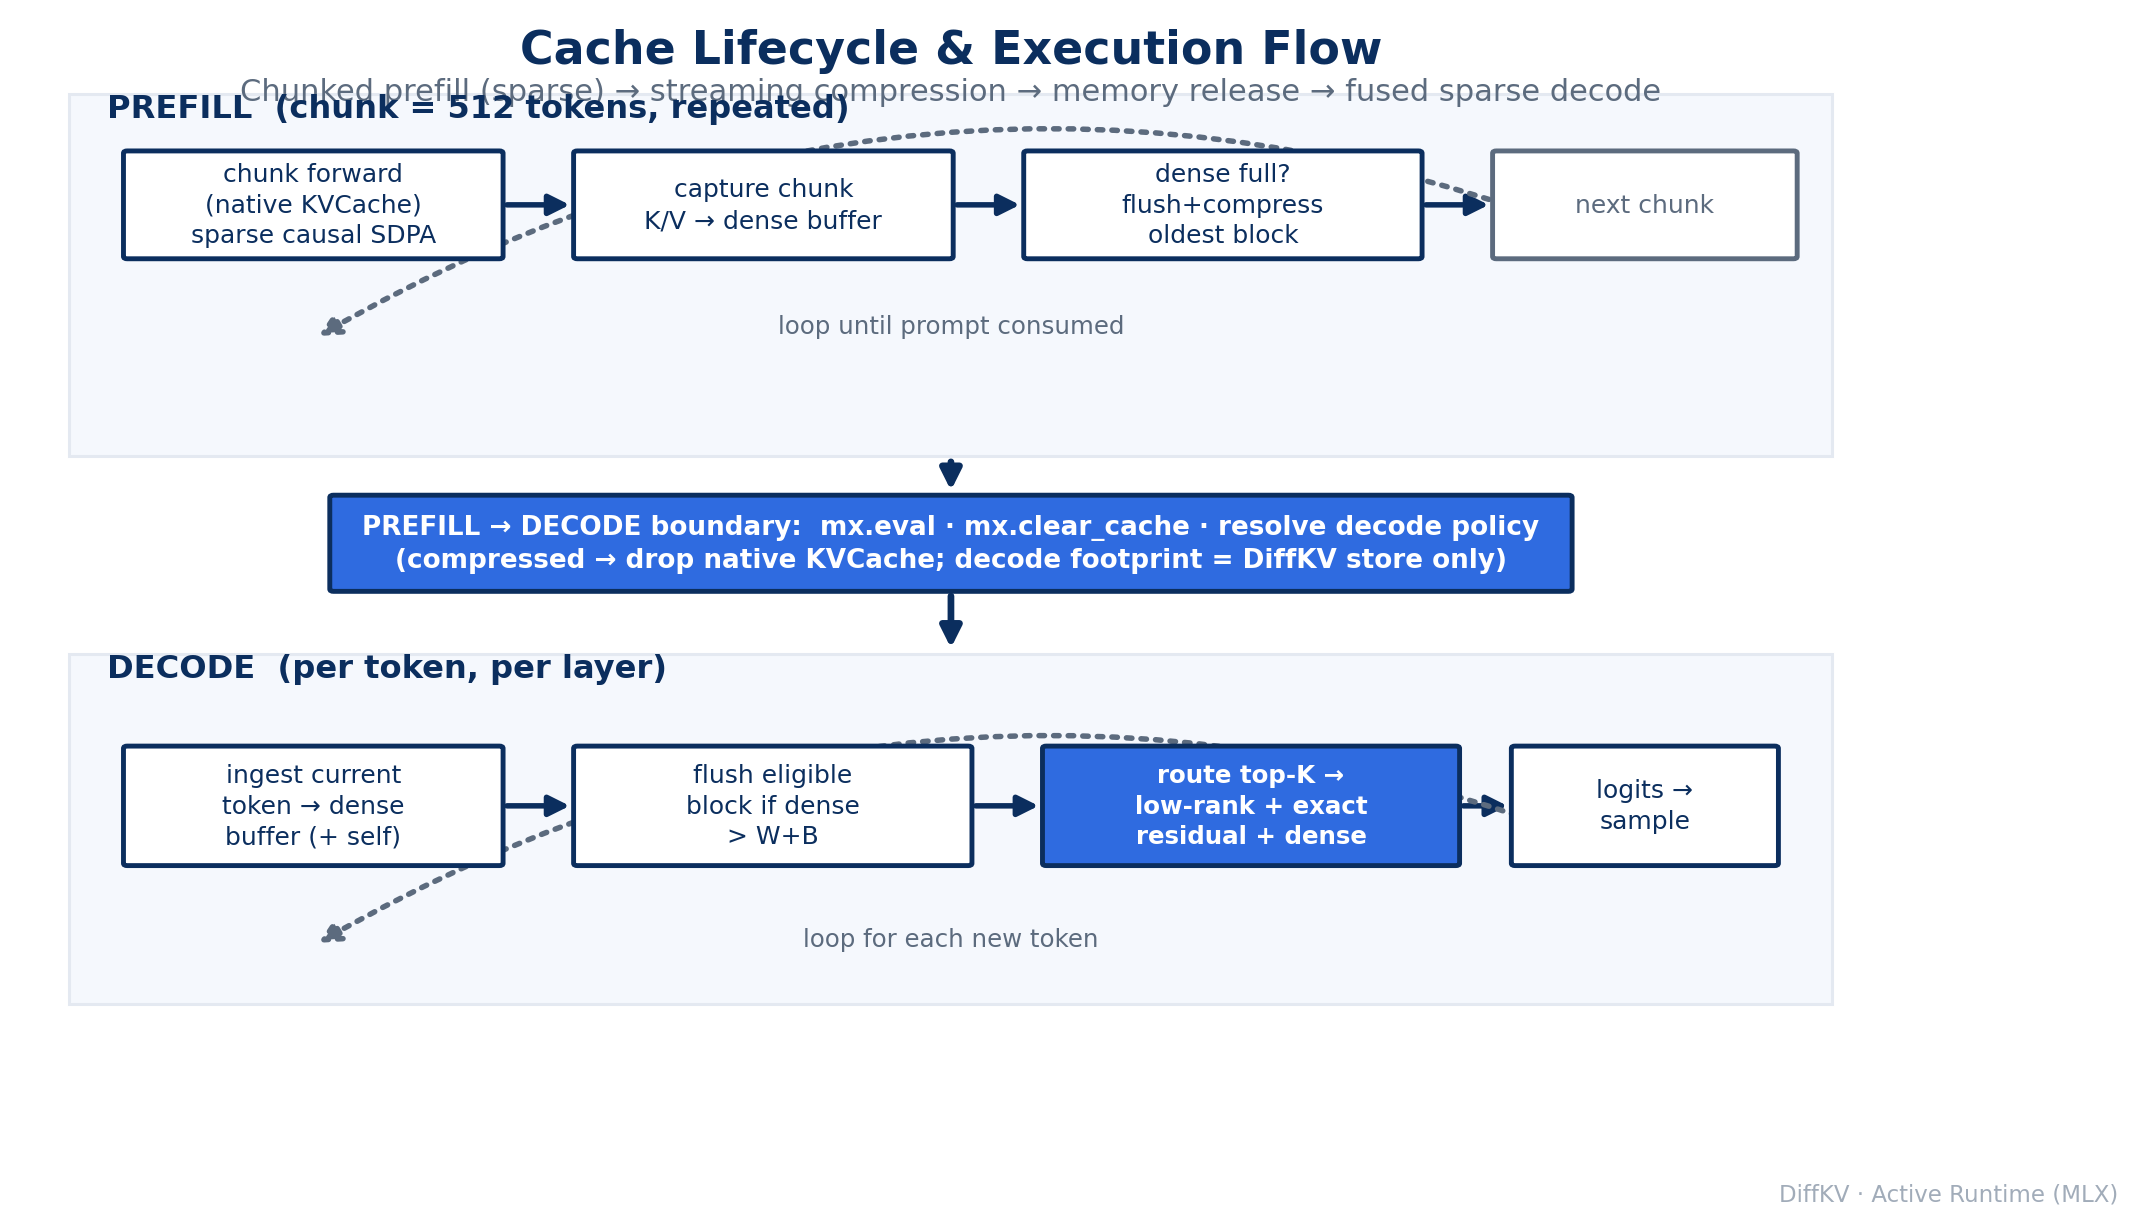
\includegraphics[width=\linewidth]{figures/f4_lifecycle.png}
  \caption{Cache lifecycle. Chunked exact prefill streams compression into the pool; the
  prefill$\to$decode boundary releases the prefill activations and drops the native cache;
  decode then ingests, compresses on overflow, and attends from the bounded store.}
  \label{fig:lifecycle}
\end{figure}

\subsection{Session lifecycle}
Beyond a single generation, the manager supports \texttt{init}/\texttt{clear},
\texttt{clone} (copy-on-write of the store and the prompt cache), \texttt{snapshot}/
\texttt{restore} (checkpointing), and \texttt{rollback} to a target length (discarding whole
compressed blocks and trimming the window). These give the serving layer multi-turn and
speculative-branching support; we list them for completeness as they define the store's
mutation API but do not evaluate them here.
